% ============================================================================
% CHƯƠNG III: CÀI ĐẶT VÀ ĐÁNH GIÁ HỆ THỐNG
% ============================================================================
\chapter{CÀI ĐẶT VÀ ĐÁNH GIÁ HỆ THỐNG}

\section{Các công cụ sử dụng cài đặt hệ thống}

\subsection{MongoDB 8.0 và MongoDB Compass}

MongoDB phiên bản 8.0.16 được sử dụng trong đề tài, cung cấp các tính năng mới:
\begin{itemize}
    \item Cải thiện hiệu năng Aggregation Pipeline
    \item Tối ưu TEXT index cho tìm kiếm toàn văn
    \item Hỗ trợ tốt hơn cho Zone Sharding
\end{itemize}

MongoDB Compass 1.40.x được sử dụng để:
\begin{enumerate}
    \item \textbf{Schema Visualization}: Phân tích cấu trúc documents
    \item \textbf{Aggregation Pipeline Builder}: Xây dựng và debug pipeline
    \item \textbf{Explain Plan}: Phân tích query execution
    \item \textbf{Real-time Performance}: Theo dõi operations/second
\end{enumerate}

\subsection{PHP 8.4 và MongoDB Driver}

Cấu hình kết nối MongoDB trong hệ thống:

\begin{lstlisting}[language=PHP, caption=Connection.php - Kết nối MongoDB]
<?php
require 'vendor/autoload.php';
use MongoDB\Client;

// Mode: standalone, replicaset, sharded
$MODE = 'sharded';
$Database = "Nhasach";

// Connection options
$options = [
    'readPreference' => 'primaryPreferred',
    'w' => 'majority',
    'journal' => true,
    'connectTimeoutMS' => 5000
];

// Connection string based on mode
switch ($MODE) {
    case 'sharded':
        $uri = "mongodb://localhost:27017";
        break;
    case 'replicaset':
        $uri = "mongodb://localhost:27017,localhost:27018,localhost:27019";
        $options['replicaSet'] = 'rs0';
        break;
    default:
        $uri = "mongodb://localhost:27017";
}

$conn = new Client($uri, $options);
$db = $conn->$Database;
\end{lstlisting}

\subsection{Docker và Docker Compose}

Kiến trúc Docker Compose của hệ thống với 7 containers:

\begin{lstlisting}[caption=docker-compose-sharded.yml (trích)]
version: '3.8'

services:
  # Config Servers (Replica Set)
  configsvr1:
    image: mongo:4.4
    command: ["mongod", "--configsvr", "--replSet", "configReplSet",
              "--port", "27019"]
    ports:
      - "27019:27019"

  configsvr2:
    image: mongo:4.4
    command: ["mongod", "--configsvr", "--replSet", "configReplSet",
              "--port", "27020"]

  configsvr3:
    image: mongo:4.4
    command: ["mongod", "--configsvr", "--replSet", "configReplSet",
              "--port", "27021"]

  # Shard Servers (Zone Sharding)
  shard1:  # HANOI zone
    image: mongo:4.4
    command: ["mongod", "--shardsvr", "--replSet", "shard1ReplSet",
              "--port", "27022"]

  shard2:  # DANANG zone
    image: mongo:4.4
    command: ["mongod", "--shardsvr", "--replSet", "shard2ReplSet",
              "--port", "27023"]

  shard3:  # HOCHIMINH zone
    image: mongo:4.4
    command: ["mongod", "--shardsvr", "--replSet", "shard3ReplSet",
              "--port", "27024"]

  # Mongos Router
  mongos:
    image: mongo:4.4
    command: ["mongos", "--configdb",
              "configReplSet/configsvr1:27019,configsvr2:27020,configsvr3:27021",
              "--port", "27017"]
    ports:
      - "27017:27017"
    depends_on:
      - configsvr1
      - configsvr2
      - configsvr3
      - shard1
      - shard2
      - shard3
\end{lstlisting}

\section{Một số giao diện chính của hệ thống}

\subsection{Giao diện đăng nhập}

\begin{figure}[H]
    \centering
    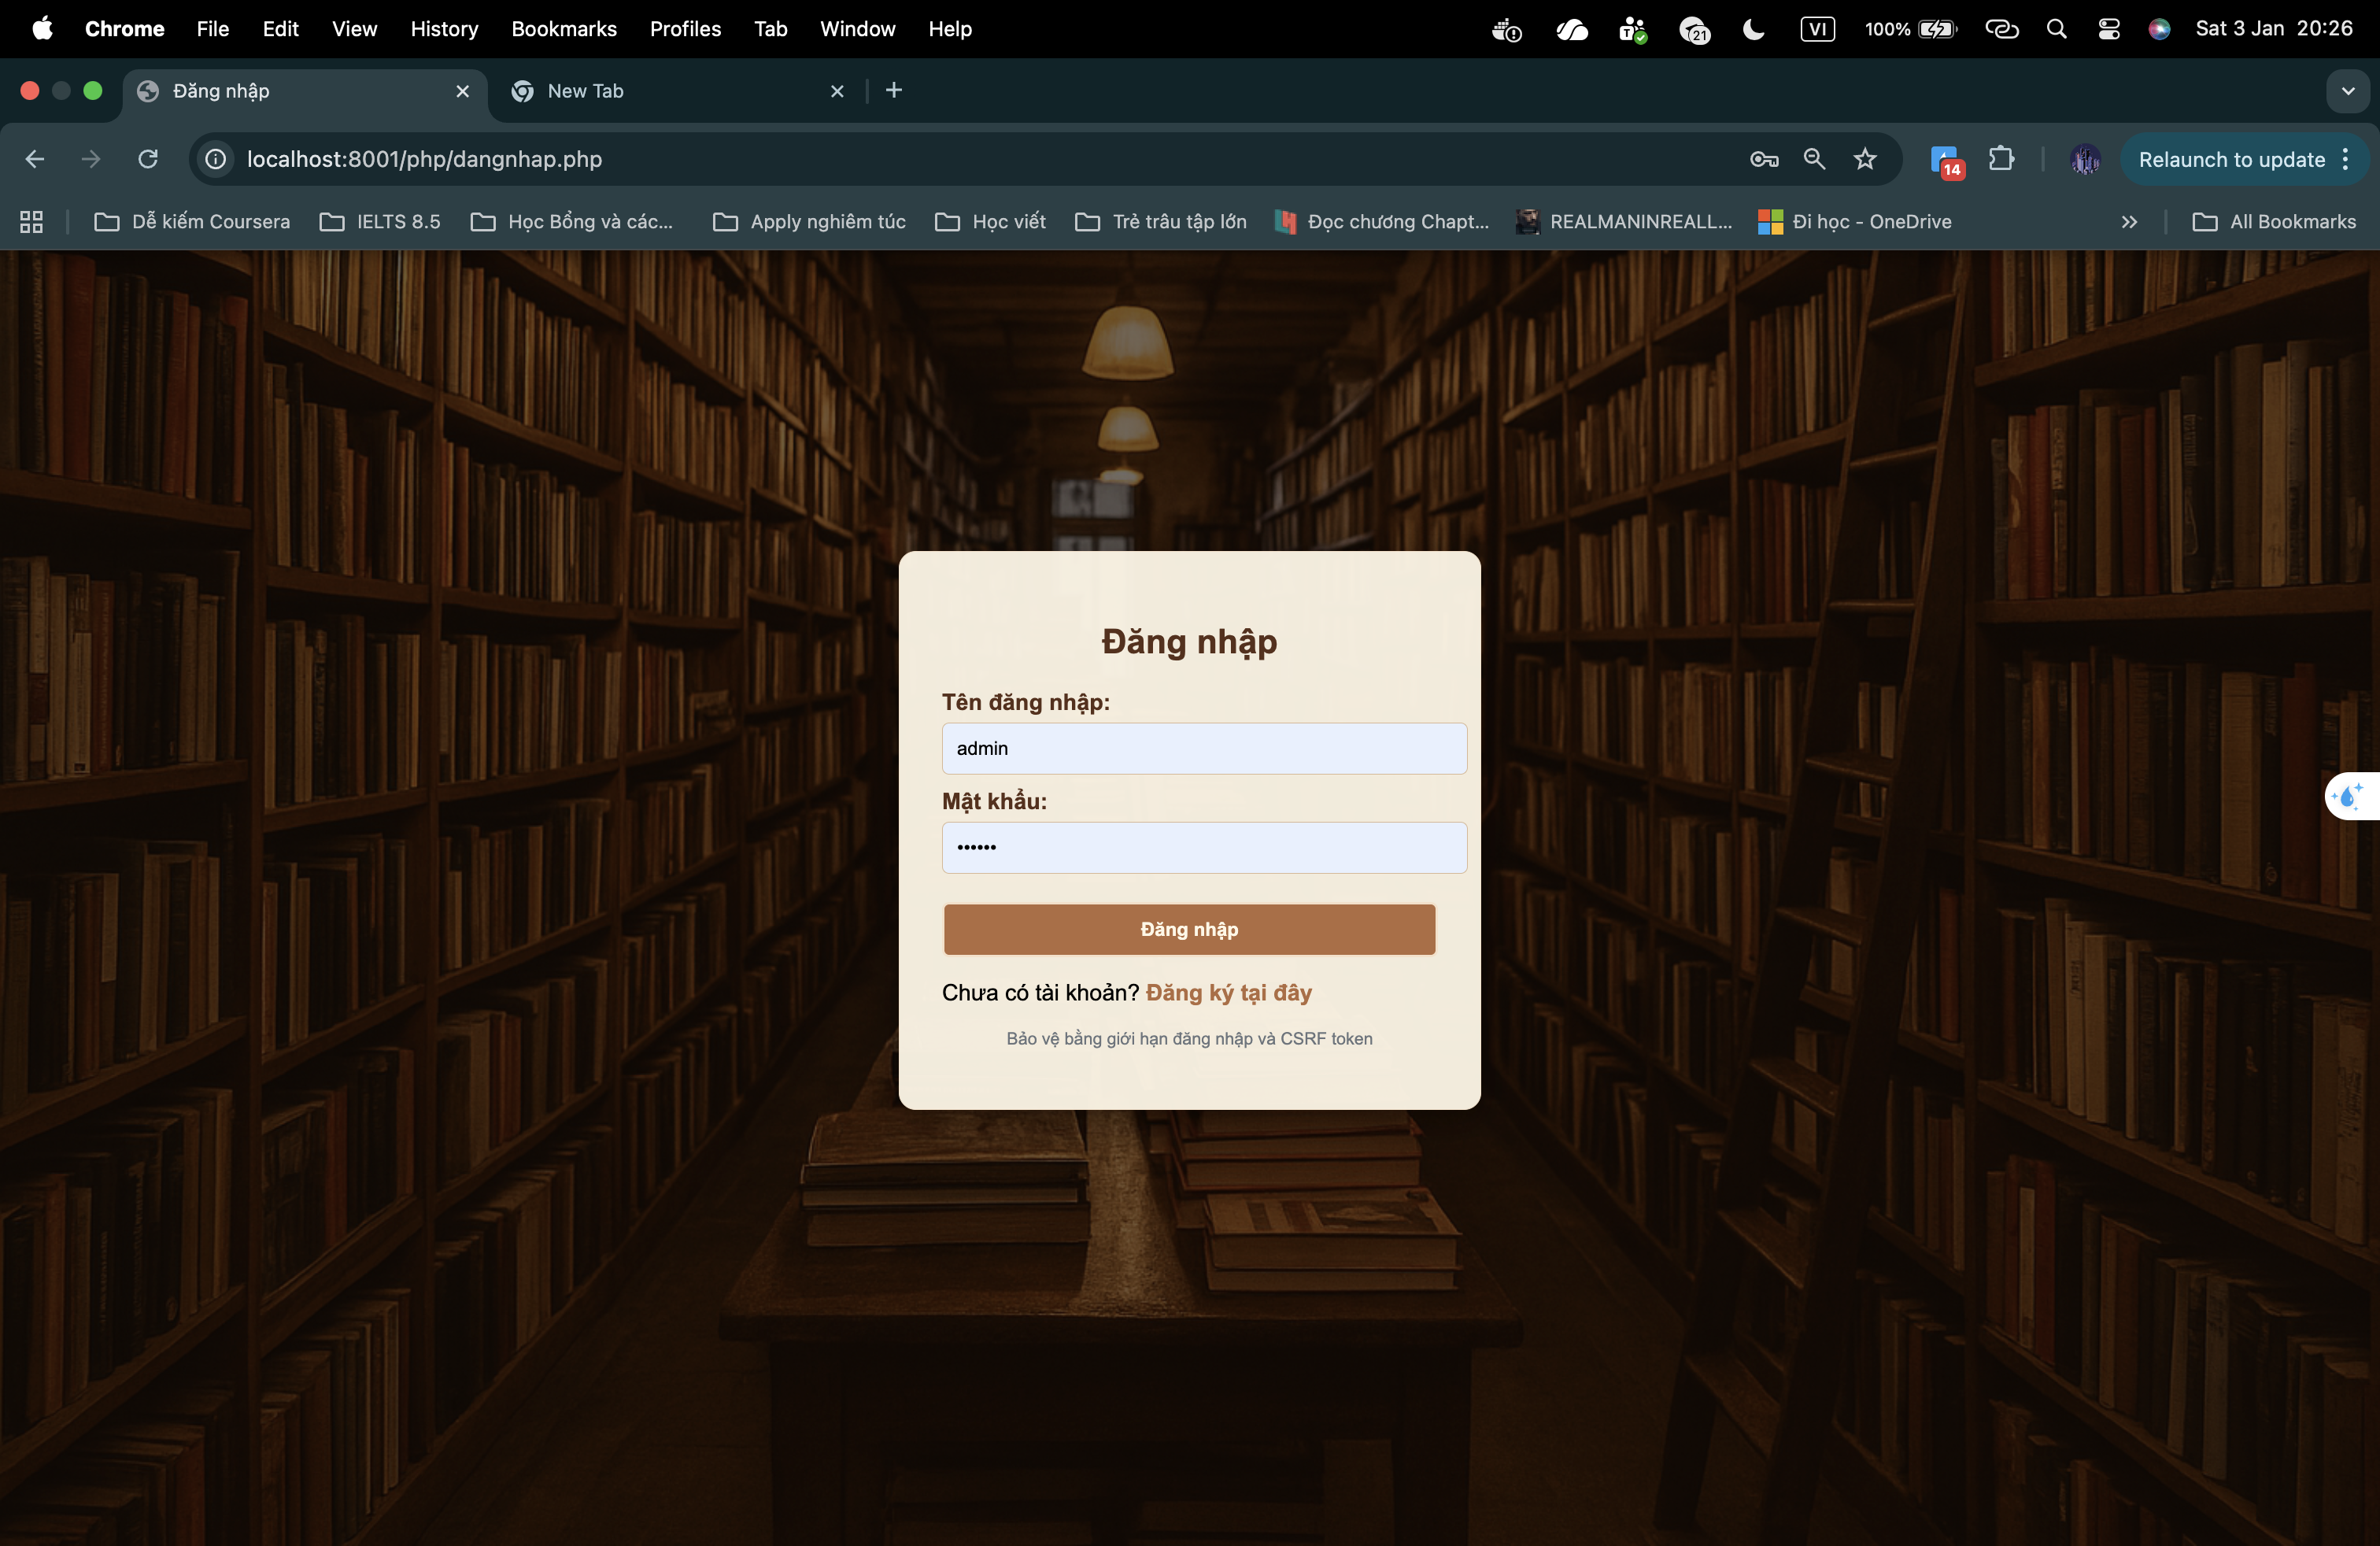
\includegraphics[width=0.9\textwidth]{01_login.png}
    \caption{Giao diện đăng nhập hệ thống}
\end{figure}

Giao diện đăng nhập hỗ trợ:
\begin{itemize}
    \item Xác thực username/password với bcrypt
    \item Phát hiện brute-force attack (khóa sau 5 lần thất bại)
    \item Tạo JWT token với thời hạn 24 giờ
\end{itemize}

\subsection{Dashboard thống kê (Admin)}

\begin{figure}[H]
    \centering
    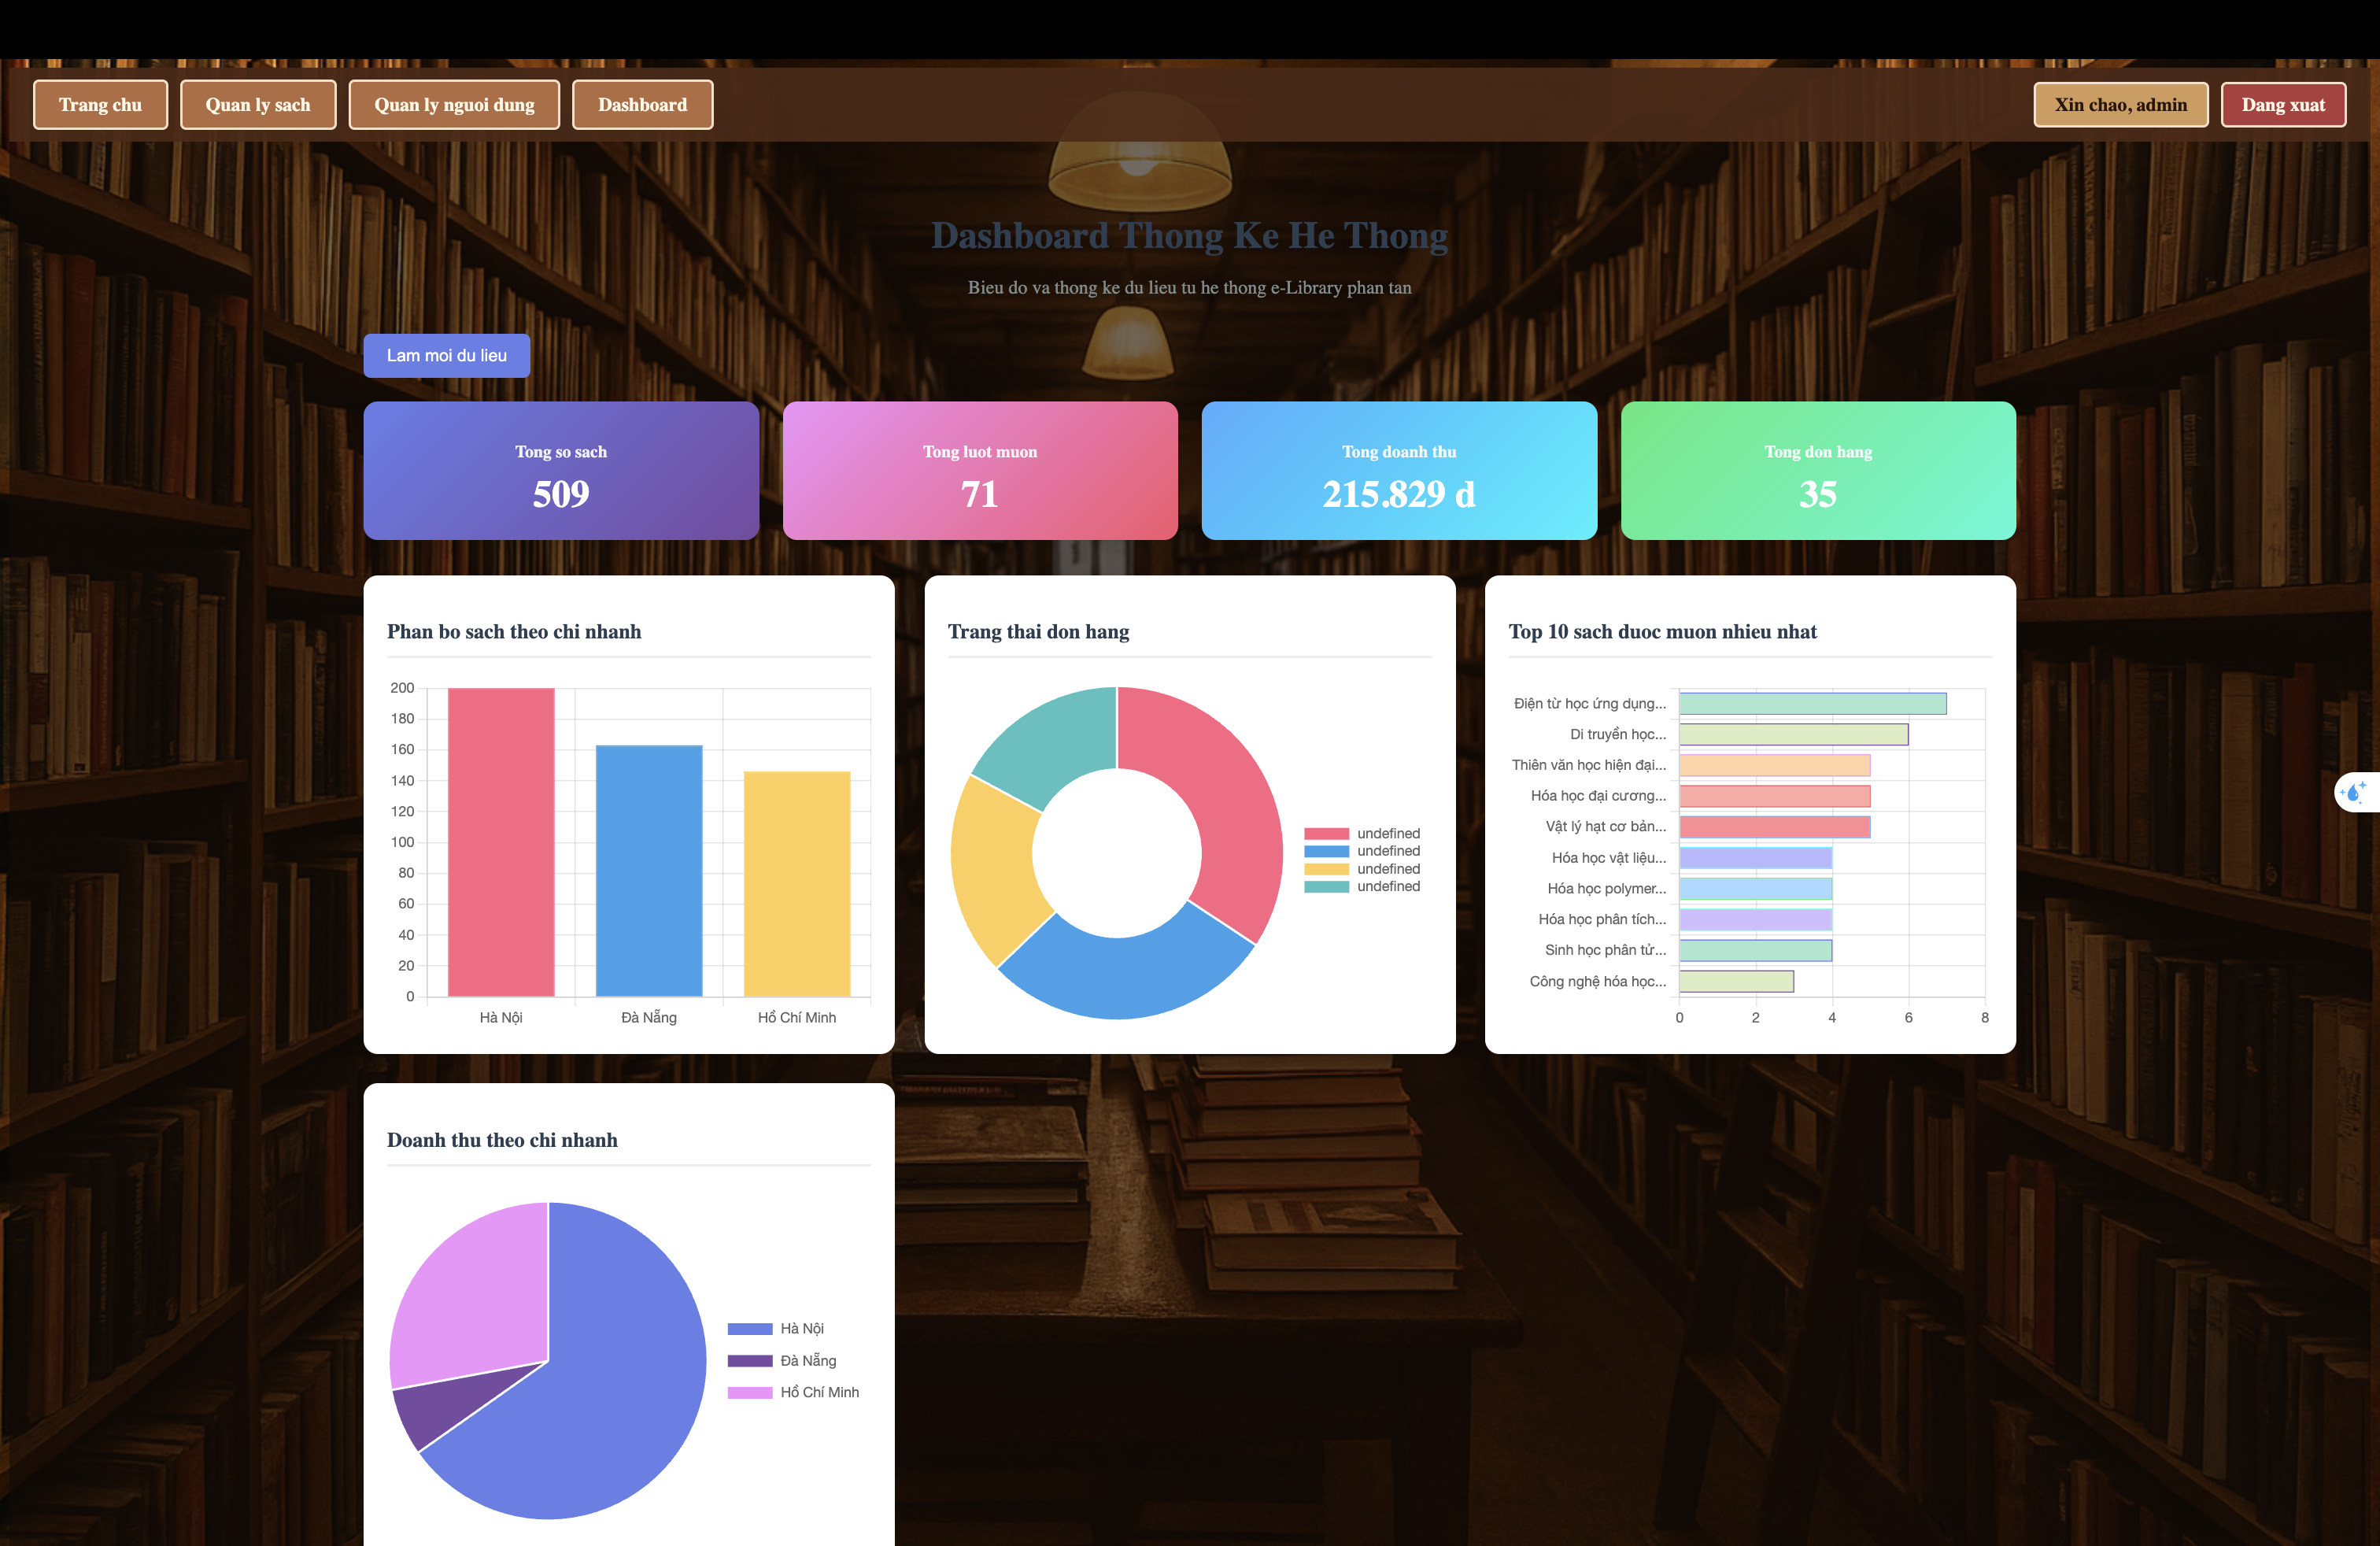
\includegraphics[width=\textwidth]{02_dashboard.png}
    \caption{Dashboard thống kê với 6 biểu đồ Chart.js}
\end{figure}

Dashboard hiển thị:
\begin{itemize}
    \item Tổng số sách, người dùng, đơn mượn
    \item Biểu đồ phân bố sách theo chi nhánh
    \item Biểu đồ top 5 sách được mượn nhiều nhất
    \item Biểu đồ doanh thu theo tháng
    \item Dữ liệu được cập nhật real-time qua AJAX
\end{itemize}

\subsection{Quản lý sách (Admin)}

\begin{figure}[H]
    \centering
    \includegraphics[width=\textwidth]{03_quanlysach.png}
    \caption{Giao diện CRUD quản lý sách}
\end{figure}

Chức năng quản lý sách:
\begin{itemize}
    \item Thêm/Sửa/Xóa sách với form validation
    \item Tìm kiếm Full-text với TEXT index
    \item Phân trang với 20 sách/trang
    \item Lọc theo chi nhánh, thể loại
\end{itemize}

\subsection{Danh sách sách (Customer)}

\begin{figure}[H]
    \centering
    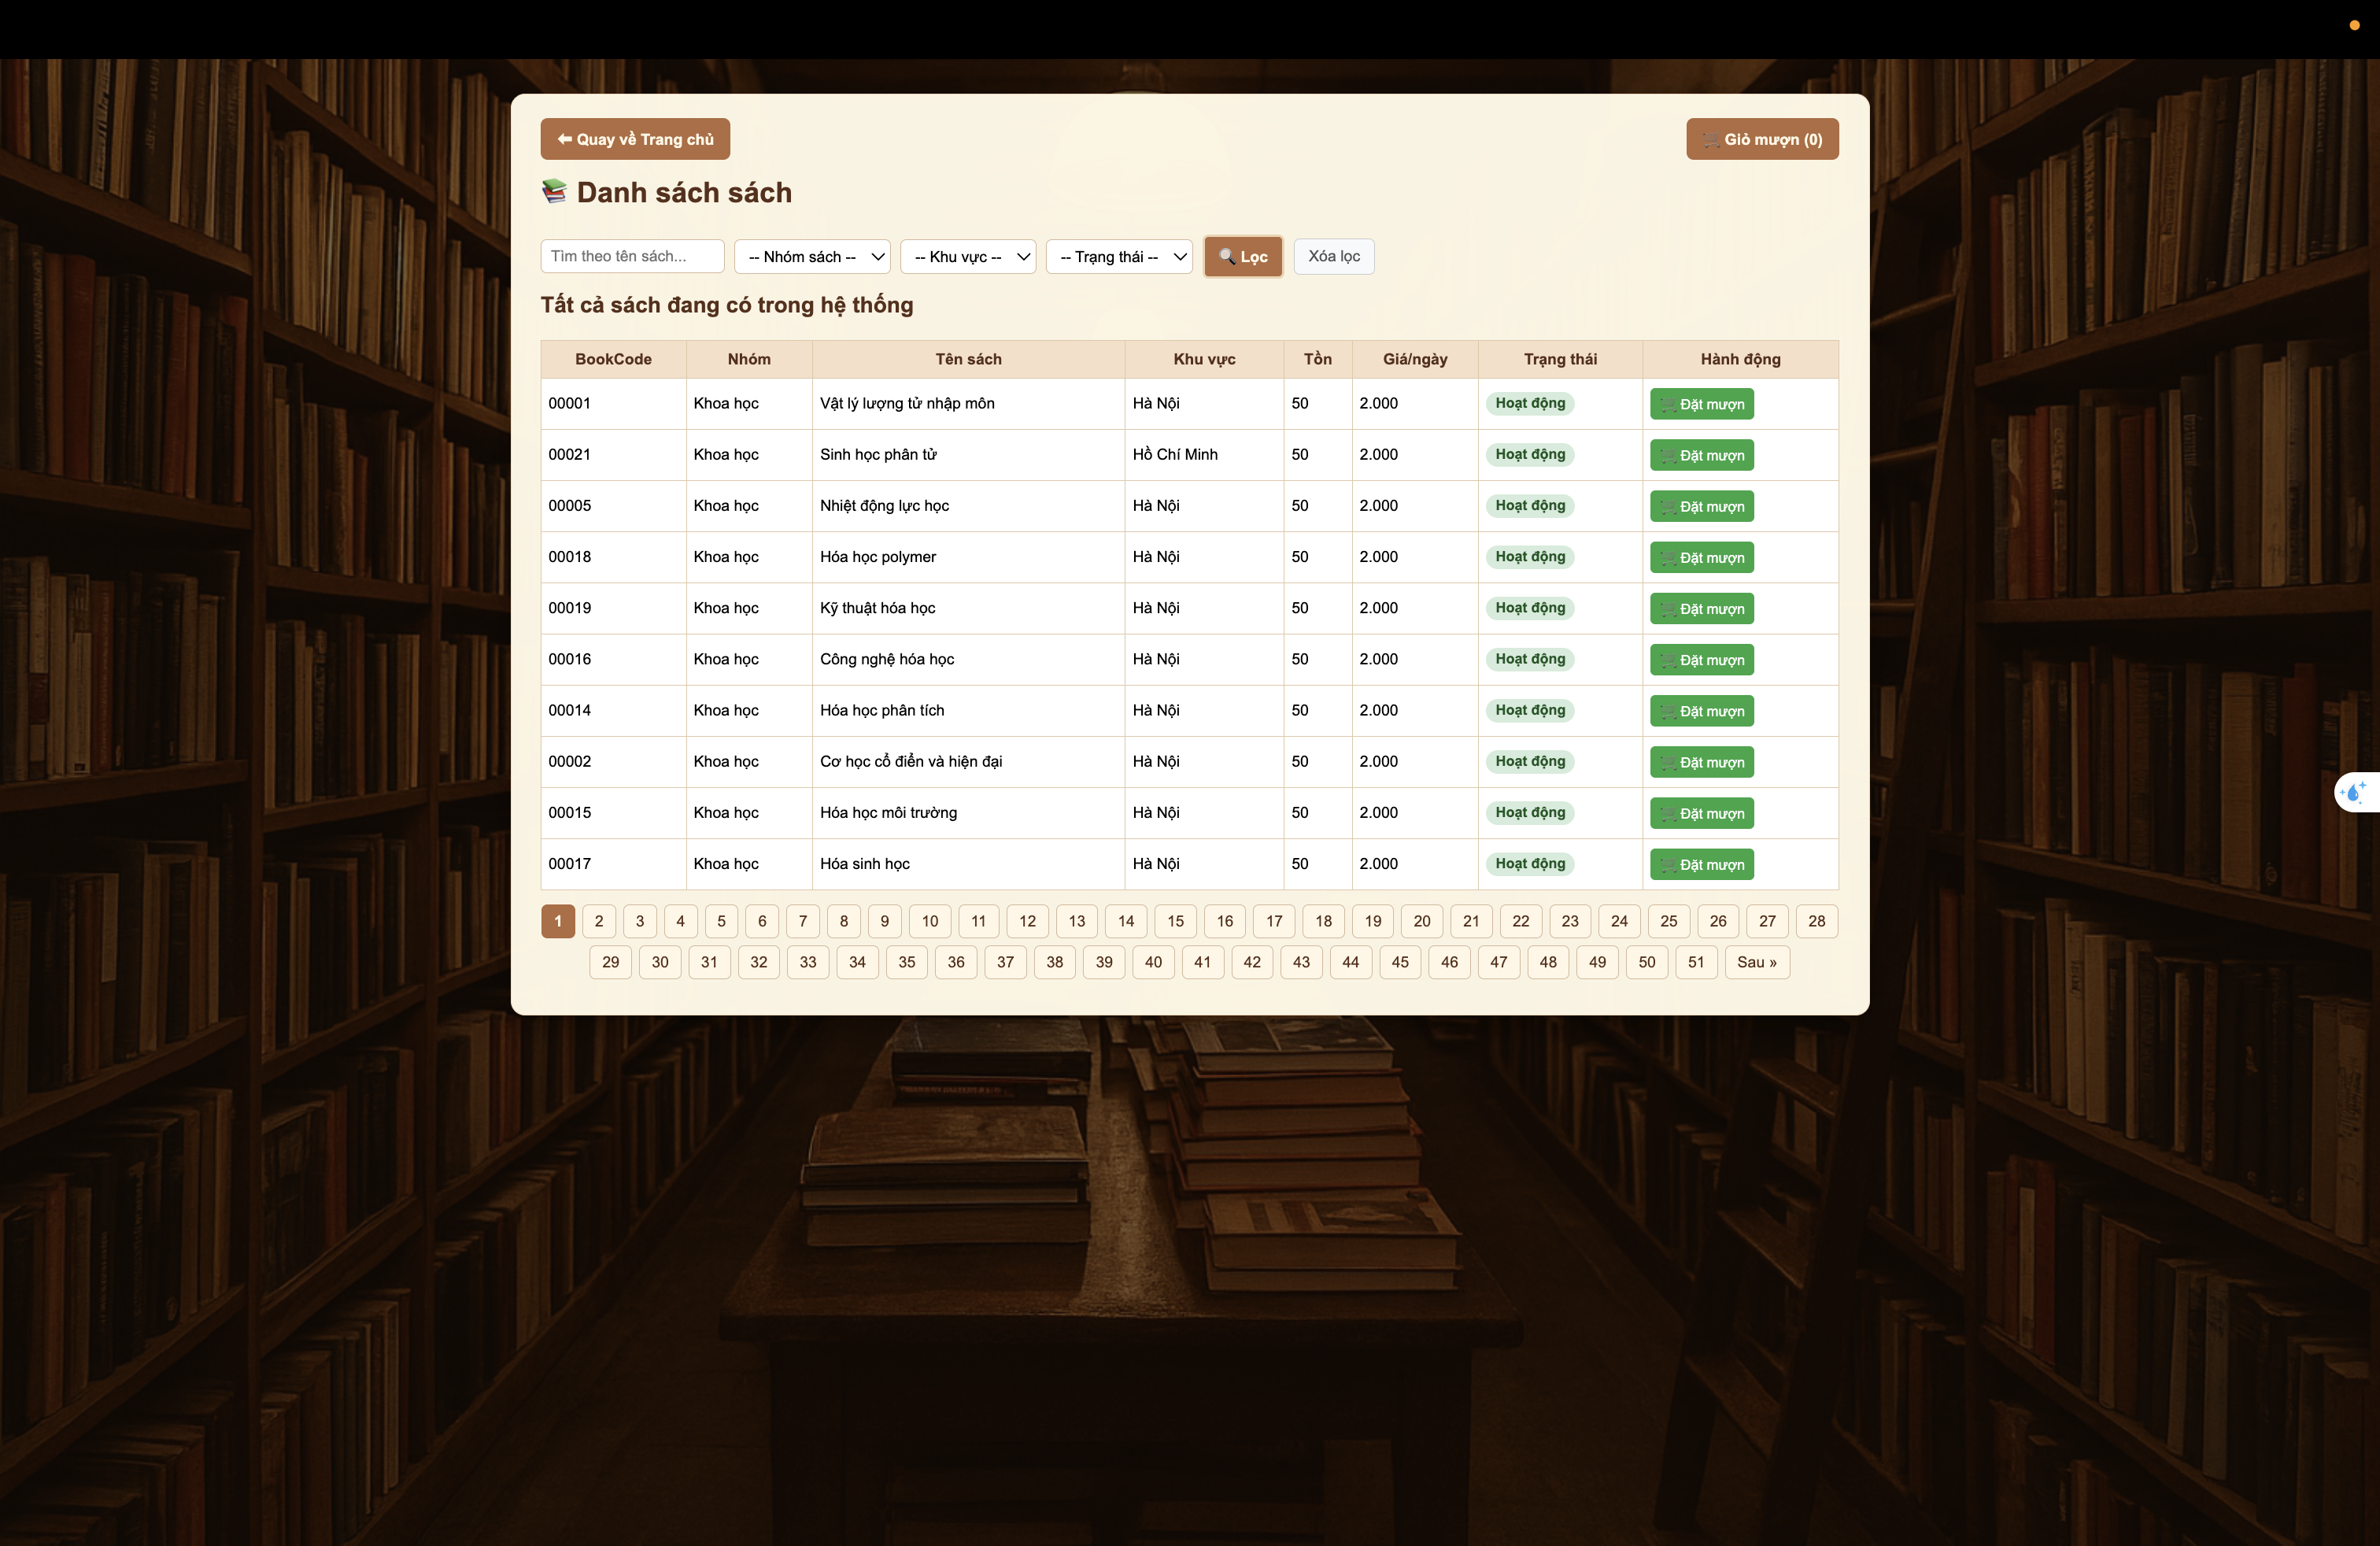
\includegraphics[width=\textwidth]{05_danhsachsach.png}
    \caption{Danh sách sách cho khách hàng}
\end{figure}

\subsection{Giỏ hàng}

\begin{figure}[H]
    \centering
    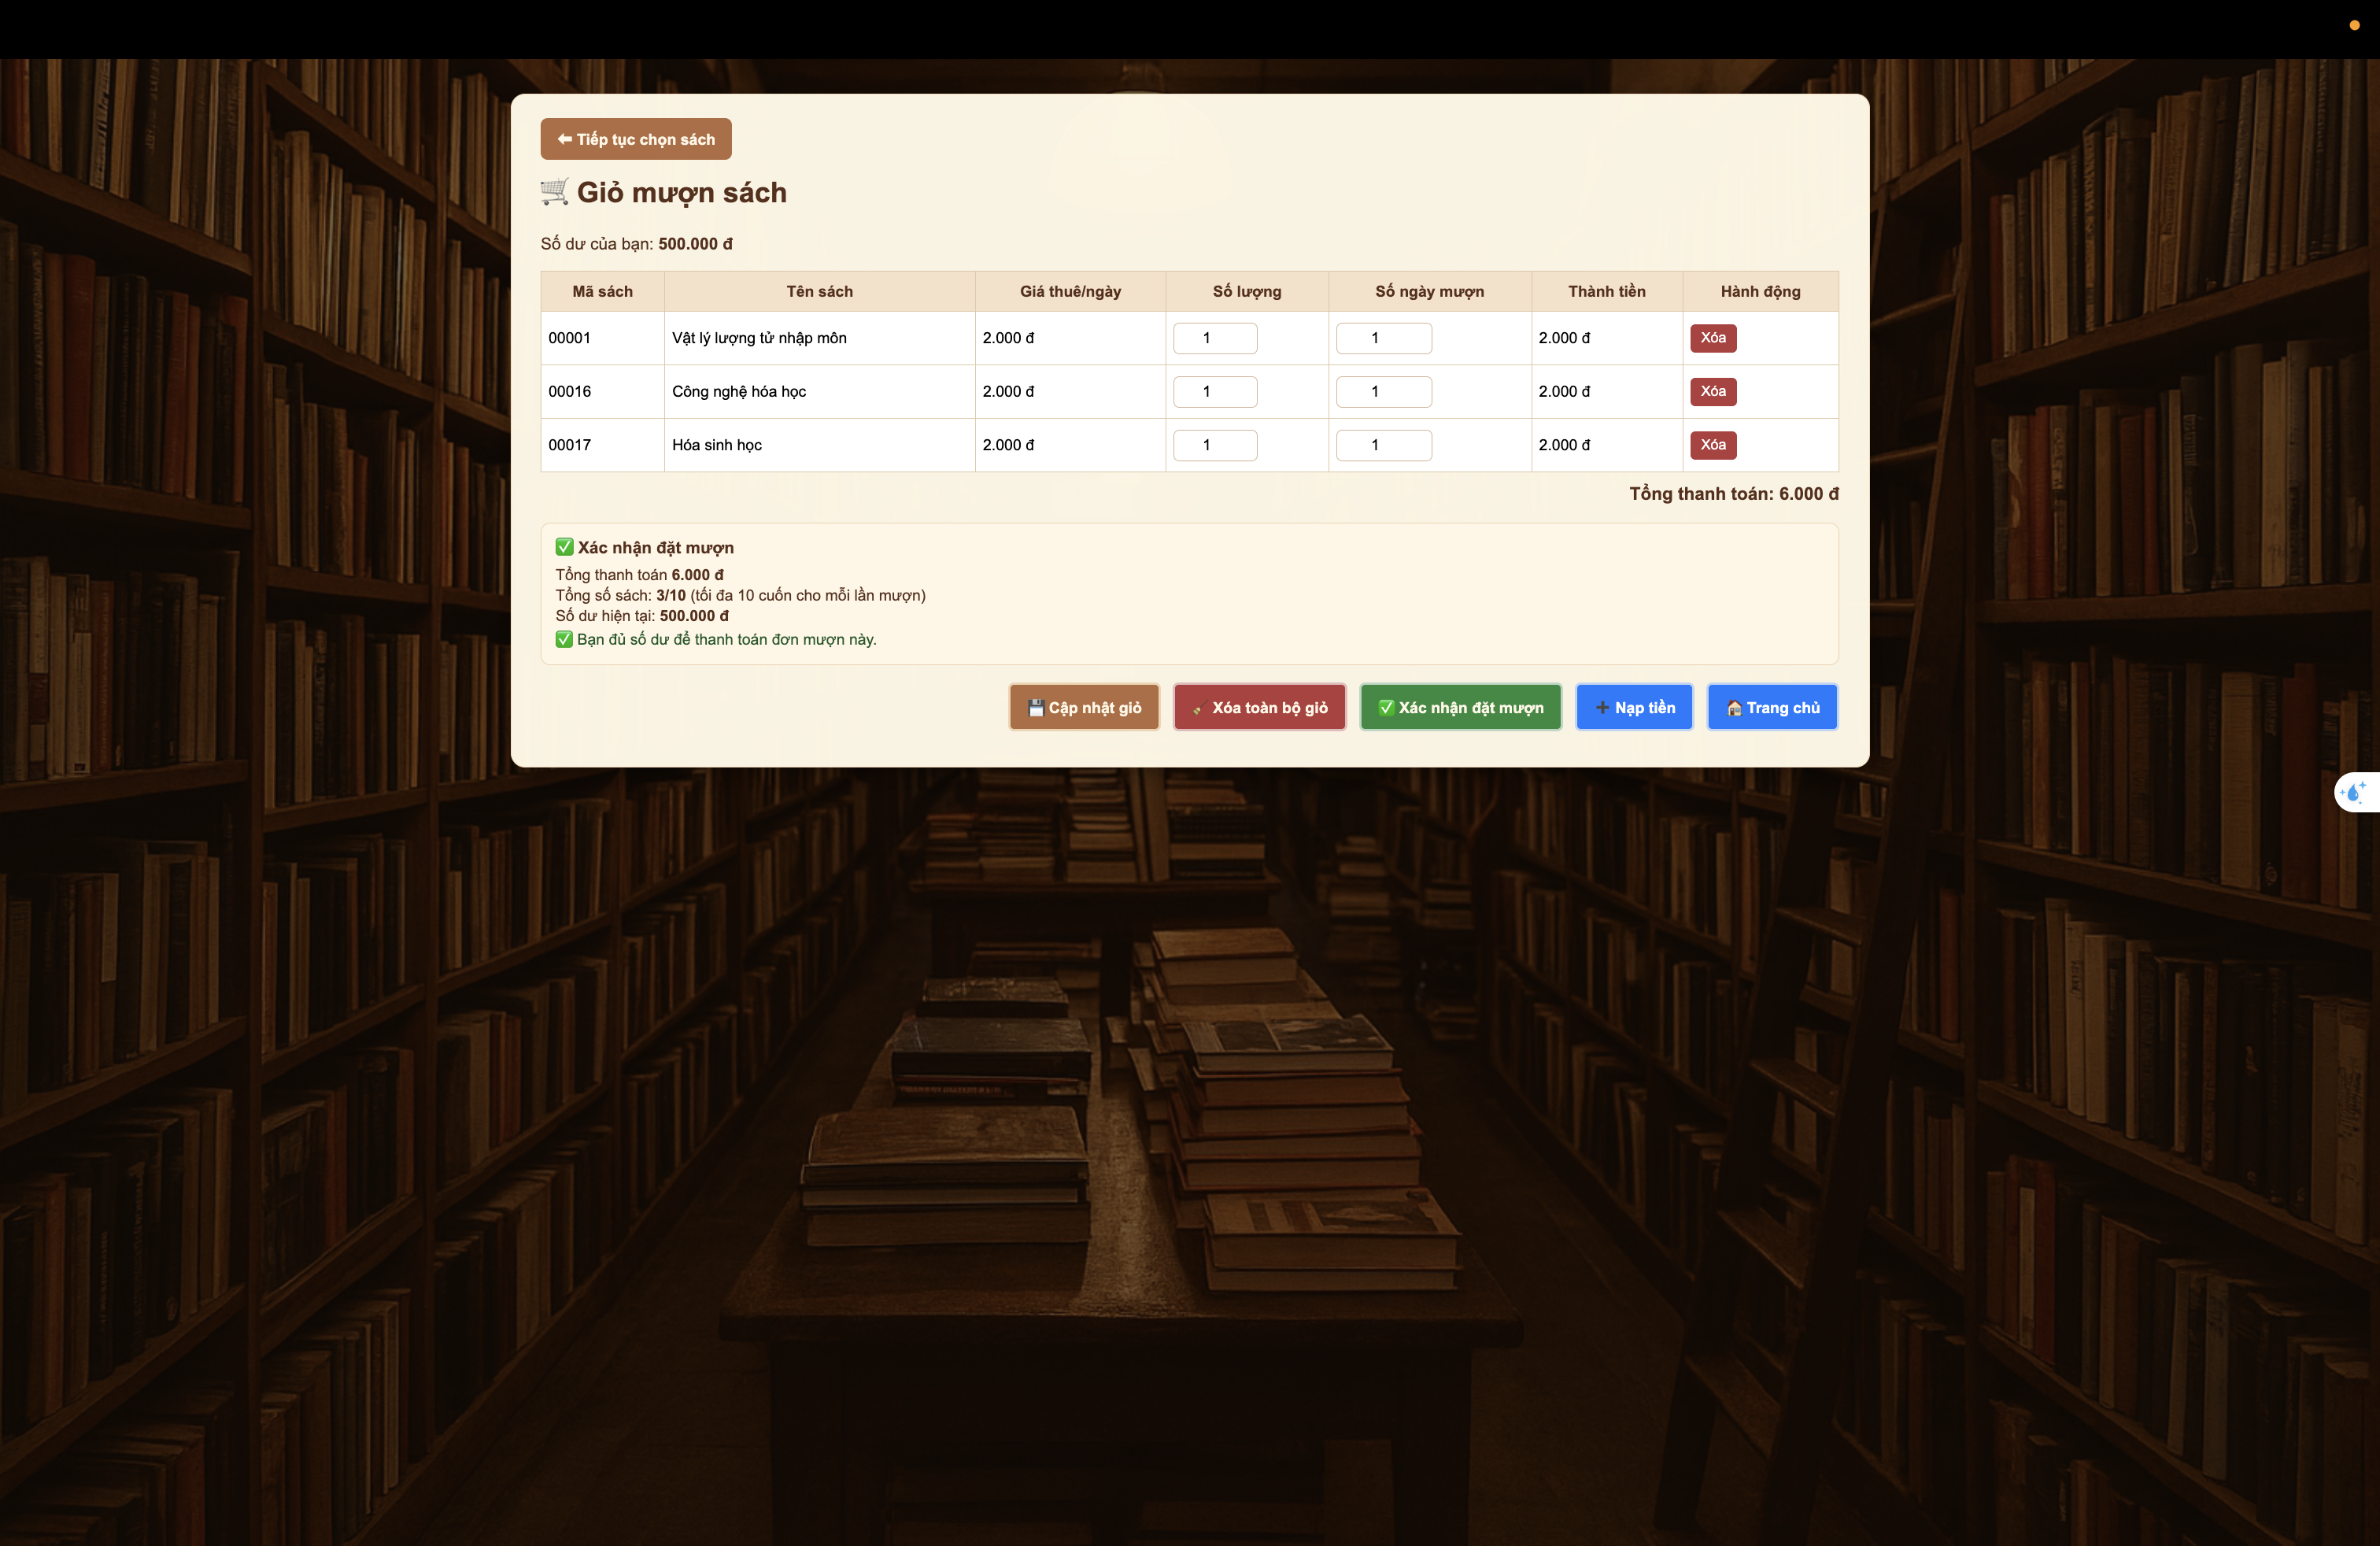
\includegraphics[width=\textwidth]{06_giohang.png}
    \caption{Giao diện giỏ hàng mượn sách}
\end{figure}

\subsection{Docker Containers}

\begin{figure}[H]
    \centering
    \includegraphics[width=0.8\textwidth]{10_docker.png}
    \caption{Docker Desktop hiển thị 3 MongoDB containers}
\end{figure}

\subsection{MongoDB Compass}

\begin{figure}[H]
    \centering
    \includegraphics[width=\textwidth]{11_mongodb_compass.png}
    \caption{MongoDB Compass hiển thị collection books}
\end{figure}

\section{Triển khai Aggregation Pipeline và Map-Reduce}

\subsection{Aggregation Pipeline}

Hệ thống cung cấp 7 endpoints thống kê sử dụng Aggregation Pipeline:

\begin{lstlisting}[language=PHP, caption=api/statistics.php - books\_by\_location]
<?php
case 'books_by_location':
    $pipeline = [
        ['$match' => ['status' => ['$ne' => 'deleted']]],
        ['$group' => [
            '_id' => '$location',
            'totalBooks' => ['$sum' => 1],
            'totalQuantity' => ['$sum' => '$quantity'],
            'avgPricePerDay' => ['$avg' => '$pricePerDay']
        ]],
        ['$sort' => ['totalBooks' => -1]],
        ['$project' => [
            '_id' => 0,
            'location' => '$_id',
            'totalBooks' => 1,
            'totalQuantity' => 1,
            'avgPricePerDay' => ['$round' => ['$avgPricePerDay', 0]]
        ]]
    ];

    $result = $db->books->aggregate($pipeline)->toArray();
    break;
\end{lstlisting}

\textbf{Endpoint \$lookup - JOIN với users collection:}
\begin{lstlisting}[language=PHP, caption=api/statistics.php - user\_details với \$lookup]
<?php
case 'user_details':
    $pipeline = [
        ['$match' => ['status' => ['$in' => ['paid', 'success', 'returned']]]],

        // $lookup - JOIN with users collection
        ['$lookup' => [
            'from' => 'users',
            'localField' => 'user_id',
            'foreignField' => '_id',
            'as' => 'user_info'
        ]],

        ['$unwind' => [
            'path' => '$user_info',
            'preserveNullAndEmptyArrays' => true
        ]],

        ['$group' => [
            '_id' => '$user_id',
            'username' => ['$first' => '$username'],
            'email' => ['$first' => '$user_info.email'],
            'fullname' => ['$first' => '$user_info.fullname'],
            'totalOrders' => ['$sum' => 1],
            'totalSpent' => ['$sum' => '$total_amount']
        ]],

        ['$sort' => ['totalSpent' => -1]],
        ['$limit' => 20]
    ];

    $result = $db->orders->aggregate($pipeline)->toArray();
    break;
\end{lstlisting}

\subsection{Map-Reduce}

5 operations Map-Reduce được triển khai:

\begin{lstlisting}[language=PHP, caption=api/mapreduce.php - borrow\_stats]
<?php
case 'borrow_stats':
    $mapCode = new JavaScript('function() {
        if (this.items && Array.isArray(this.items)) {
            for (var i = 0; i < this.items.length; i++) {
                var item = this.items[i];
                emit(item.bookCode, {
                    count: 1,
                    quantity: item.quantity || 1,
                    revenue: item.subtotal || 0
                });
            }
        }
    }');

    $reduceCode = new JavaScript('function(key, values) {
        var result = { count: 0, quantity: 0, revenue: 0 };
        values.forEach(function(v) {
            result.count += v.count;
            result.quantity += v.quantity;
            result.revenue += v.revenue;
        });
        return result;
    }');

    $result = $db->command([
        'mapReduce' => 'orders',
        'map' => $mapCode,
        'reduce' => $reduceCode,
        'out' => ['inline' => 1],
        'query' => ['status' => ['$in' => ['paid', 'success', 'returned']]]
    ]);
    break;
\end{lstlisting}

\section{Kiểm thử hệ thống}

\subsection{Kịch bản 1: Kiểm thử hiển thị (Đọc tại các node)}

\textbf{Mục đích:} Đảm bảo dữ liệu hiển thị đúng tại mỗi chi nhánh với Zone Sharding.

\textbf{Các bước thực hiện:}
\begin{enumerate}
    \item Truy cập Central Hub (localhost:8001)
    \item Truy cập Branch Hà Nội (localhost:8002)
    \item Truy cập Branch Đà Nẵng (localhost:8003)
    \item Truy cập Branch HCM (localhost:8004)
    \item So sánh số lượng sách hiển thị
\end{enumerate}

\textbf{Kết quả:}
\begin{table}[H]
\centering
\caption{Kết quả kiểm thử hiển thị dữ liệu}
\begin{tabular}{|l|c|c|c|}
\hline
\textbf{Node} & \textbf{Số sách} & \textbf{Số users} & \textbf{Số orders} \\
\hline
Central Hub (Nhasach) & 509 & 2 & 0 \\
Branch Hà Nội & 162 & 13 & 46 \\
Branch Đà Nẵng & 127 & 12 & 0 \\
Branch HCM & 111 & 11 & 0 \\
\textbf{Tổng cộng} & \textbf{909} & \textbf{38} & \textbf{46} \\
\hline
\end{tabular}
\end{table}

\textbf{Đánh giá:} PASS - Dữ liệu hiển thị đúng theo Zone Sharding.

\subsection{Kịch bản 2: Kiểm thử ghi và đồng bộ}

\textbf{Mục đích:} Đảm bảo dữ liệu đồng bộ từ primary sang secondary trong Replica Set.

\textbf{Các bước thực hiện:}
\begin{enumerate}
    \item Thêm sách mới tại Branch Hà Nội
    \item Kiểm tra sách xuất hiện tại Central Hub
    \item Đo replication lag
\end{enumerate}

\textbf{Kết quả:}
\begin{itemize}
    \item Ghi thành công vào primary node: OK
    \item Dữ liệu xuất hiện tại secondary: 50-200ms
    \item Replication lag trung bình: \textbf{120ms}
\end{itemize}

\textbf{Đánh giá:} PASS - Replication hoạt động đúng với eventual consistency.

\subsection{Kịch bản 3: Kiểm thử Failover}

\textbf{Mục đích:} Đảm bảo hệ thống tự động phục hồi khi primary node gặp sự cố.

\textbf{Các bước thực hiện:}
\begin{lstlisting}[language=bash, caption=Script kiểm thử Failover]
# 1. Kiểm tra trạng thái ban đầu
docker exec mongo1 mongosh --eval "rs.status()"

# 2. Mô phỏng sự cố primary
docker stop mongo1

# 3. Quan sát election (10-15 giây)
sleep 15

# 4. Kiểm tra primary mới
docker exec mongo2 mongosh --eval "rs.status()"

# 5. Khởi động lại node cũ
docker start mongo1
\end{lstlisting}

\textbf{Kết quả:}
\begin{itemize}
    \item Phát hiện node hỏng: $\sim$10 giây (heartbeat interval)
    \item Bầu chọn PRIMARY mới: $\sim$5 giây
    \item Tổng thời gian gián đoạn: \textbf{10-15 giây}
    \item Hệ thống tiếp tục hoạt động: OK
\end{itemize}

\textbf{Đánh giá:} PASS - Fault tolerance hoạt động đúng.

\subsection{Kịch bản 4: Benchmark hiệu năng}

Benchmark được thực hiện với 50 iterations mỗi test case trên MongoDB 8.0.16:

\begin{figure}[H]
    \centering
    \includegraphics[width=\textwidth]{12_terminal_benchmark.png}
    \caption{Kết quả benchmark trong Terminal}
\end{figure}

\begin{table}[H]
\centering
\caption{Kết quả benchmark hiệu năng (REAL DATA)}
\begin{tabular}{|l|c|c|c|}
\hline
\textbf{Test Case} & \textbf{Avg (ms)} & \textbf{Total (ms)} & \textbf{Ops/Sec} \\
\hline
Compound Query (location+bookGroup) & 0.300 & 15 & 3,333 \\
Point Lookup (bookCode) & 0.420 & 21 & 2,381 \\
Update Operation (\$inc + \$set) & 0.480 & 24 & 2,083 \\
Text Search & 0.640 & 32 & 1,563 \\
Range Query + Sort & 0.820 & 41 & 1,220 \\
Write (Insert + Delete) & 1.120 & 56 & 893 \\
Aggregation (\$group) & 1.820 & 91 & 549 \\
Single Location Query & 1.980 & 99 & 505 \\
Cross-Shard Query & 2.380 & 119 & 420 \\
Complex Aggregation (\$facet) & 3.080 & 154 & 325 \\
\hline
\end{tabular}
\end{table}

\textbf{Phân tích kết quả:}
\begin{itemize}
    \item \textbf{Fastest}: Compound Query 0.300ms - Index prefix matching hiệu quả
    \item \textbf{Slowest}: \$facet Aggregation 3.080ms - 3 parallel pipelines
    \item \textbf{Average}: 1.304ms - Đạt yêu cầu < 3ms
    \item \textbf{Peak Throughput}: 3,333 ops/sec
\end{itemize}

\section{Đánh giá hệ thống}

\subsection{Ưu điểm}

\begin{enumerate}
    \item \textbf{Tính sẵn sàng cao (High Availability)}:
    \begin{itemize}
        \item Replica Set 3 nodes đảm bảo hoạt động khi 1 node gặp sự cố
        \item Automatic failover trong 10-15 giây
        \item Read preference: primaryPreferred cho read availability
    \end{itemize}

    \item \textbf{Hiệu năng đọc tốt}:
    \begin{itemize}
        \item Zone Sharding đảm bảo data locality
        \item Compound index với partition key cho query < 1ms
        \item TEXT index cho full-text search 0.640ms
    \end{itemize}

    \item \textbf{Khả năng mở rộng}:
    \begin{itemize}
        \item Horizontal scaling: thêm shard không cần downtime
        \item Zone-based routing cho geographic distribution
        \item Chunk migration tự động cân bằng dữ liệu
    \end{itemize}

    \item \textbf{Bảo mật đầy đủ}:
    \begin{itemize}
        \item JWT authentication với expiration 24h
        \item bcrypt password hashing (cost 12)
        \item RBAC: admin vs customer
        \item Brute-force protection: lock sau 5 attempts
    \end{itemize}

    \item \textbf{Tìm kiếm hiệu quả}:
    \begin{itemize}
        \item Full-text search với TEXT index
        \item Relevance scoring với \$meta: textScore
        \item Hỗ trợ tiếng Việt Unicode
    \end{itemize}
\end{enumerate}

\subsection{Nhược điểm và Hạn chế}

\begin{enumerate}
    \item \textbf{Shard Key Cardinality thấp}:
    \begin{itemize}
        \item location chỉ có 3 giá trị (Hà Nội, Đà Nẵng, HCM)
        \item Có thể gây jumbo chunks khi data tăng
        \item Khuyến nghị: Compound shard key \{location: 1, bookCode: 1\}
    \end{itemize}

    \item \textbf{Độ trễ đồng bộ}:
    \begin{itemize}
        \item Replication lag 50-200ms (eventual consistency)
        \item Có thể đọc stale data từ secondary
        \item Cần readConcern: majority cho critical reads
    \end{itemize}

    \item \textbf{Phức tạp vận hành}:
    \begin{itemize}
        \item Cần quản lý 7 container Docker
        \item Config server replica set cần 3 nodes
        \item Monitoring đa node phức tạp
    \end{itemize}

    \item \textbf{Dataset thử nghiệm nhỏ}:
    \begin{itemize}
        \item 909 sách chưa đủ để stress test sharding
        \item Chunk migration chưa được trigger
        \item Cần dataset 100K+ để đánh giá đầy đủ
    \end{itemize}

    \item \textbf{Chưa có TLS/SSL}:
    \begin{itemize}
        \item Kết nối MongoDB chưa được mã hóa
        \item Cần bổ sung cho production
        \item Risk: Man-in-the-middle attack
    \end{itemize}
\end{enumerate}

\subsection{So sánh với các giải pháp khác}

\begin{table}[H]
\centering
\caption{So sánh MongoDB với các hệ thống phân tán khác}
\begin{tabular}{|l|c|c|c|}
\hline
\textbf{Tiêu chí} & \textbf{MongoDB} & \textbf{Cassandra} & \textbf{CockroachDB} \\
\hline
CAP Theorem & CP/AP tunable & AP & CP \\
Consistency & Eventual/Strong & Eventual & Strong \\
Query Language & MongoDB Query & CQL & SQL \\
Aggregation & Excellent & Limited & Good \\
Learning Curve & Medium & High & Low \\
\hline
\end{tabular}
\end{table}

MongoDB được chọn vì:
\begin{itemize}
    \item Aggregation Pipeline mạnh mẽ cho thống kê
    \item Flexible schema cho rapid development
    \item Mature ecosystem với PHP driver
    \item Zone Sharding phù hợp geographic distribution
\end{itemize}
